
%(BEGIN_QUESTION)
% Copyright 2007, Tony R. Kuphaldt, released under the Creative Commons Attribution License (v 1.0)
% This means you may do almost anything with this work of mine, so long as you give me proper credit

As fluid flows past a stationary object such as a {\it Pitot tube}, the fluid immediately in front of the tube comes to a full stop.  This is called a {\it stagnation point}, and the pressure resulting from the complete loss of velocity at the stagnation point is called the {\it stagnation pressure}.

$$\includegraphics[width=15.5cm]{i02981x01.eps}$$

Manipulate Bernoulli's equation to show how this stagnation pressure is determined by fluid velocity ($v$).

\underbar{file i02981}
%(END_QUESTION)





%(BEGIN_ANSWER)

\noindent
{\bf Bernoulli's equation:}

$$z_1 \rho g + {v_1^2 \rho \over 2} + P_1 = z_2 \rho g + {v_2^2 \rho \over 2} + P_2$$

Assuming no change in height ($z$) is involved:

$${v_1^2 \rho \over 2} + P_1 = {v_2^2 \rho \over 2} + P_2$$

Knowing that $P_1$ is the static pressure and that $P_2$ is equal to $P_{static}$ + $P_{stagnation}$:

$${v_1^2 \rho \over 2} + P_{static} = {v_2^2 \rho \over 2} + P_{static} + P_{stagnation}$$

$${v_1^2 \rho \over 2} = {v_2^2 \rho \over 2} + P_{stagnation}$$

Knowing that $v_2$ is zero at the stagnation point:

$${v_1^2 \rho \over 2} = P_{stagnation}$$

\vskip 10pt

Therefore, $P_{stagnation} = {1 \over 2} v^2 \rho$


%(END_ANSWER)





%(BEGIN_NOTES)

%INDEX% Measurement, flow: Pitot tube
%INDEX% Physics, dynamic fluids: Bernoulli's equation

%(END_NOTES)


